\documentclass[c,unicode,russian]{beamer}
\usepackage{hyperref}
\usepackage{alltt}
\usepackage{verbatim}
\usepackage{fancyvrb}

\usepackage{fontspec}
\setsansfont{Ubuntu}
\setmonofont{Ubuntu Mono}
\usepackage{polyglossia}
\setdefaultlanguage{russian}

\useinnertheme{metropolis}
\useoutertheme{metropolis}
\usecolortheme{metropolis}

\usepackage{listings}   % C++ code
\usepackage{xcolor}     % C++ code
\lstset{%
    keywordstyle=\color{blue},
    commentstyle=\color[rgb]{0.13,0.54,0.13},
    backgroundcolor=\color{yellow!10},
    basicstyle=\small\tt,
    stringstyle=\color{red}\ttfamily,
    belowcaptionskip=-1pt,
    xleftmargin=-15pt,
    framexleftmargin=-15pt,
    framexrightmargin=5pt,
    framextopmargin=5pt,
    framexbottommargin=5pt,
    framesep=0pt,
    rulesep=0pt
}
\lstdefinestyle{cpp}{%
    language=C++,
    morecomment=[l][\color{magenta}]{\#}
}
\lstdefinestyle{python}{%
    language=Python
}

\usepackage{caption}
\renewcommand{\lstlistingname}{Код} % Listing -> Algorithm
\DeclareCaptionFont{white}{\color{white}}
\DeclareCaptionFormat{listing}{\colorbox{gray}{\parbox{\textwidth}{#1#2#3}}}
\captionsetup[lstlisting]{format=listing,labelfont=white,textfont=white}

% logo of my university
\titlegraphic{\hspace{-1cm}
\includegraphics[width=2.5in]{../../_static/logo.jpg}}

\date{}
\author{Основы Веб-программирования}
\institute{Кафедра Интеллектуальных Информационных Технологий, ИнФО, УрФУ}


\title{HTTP}

\begin{document}

% Slide #1
\frame{\titlepage}

% Slide #2
\begin{frame}
    \frametitle{Ресурсы}
    \url{http://lectureskpd.readthedocs.org/kpd/3.http.html}
    \url{https://tools.ietf.org/html/rfc2616}
\end{frame}

% Slide #3
\begin{frame}
    \frametitle{Особенности}
    \begin{itemize}
        \item Через него передается основная часть Веб трафика
        \item Создавался для передачи HTML
        \item Сейчас используется для передачи любых данных
        \item Текстовый протокол
        \item 4го (прикладного) уровня стека протоколов TCP/IP
        \item Использует TCP соединение
        \item Может выполнить несколько запросов в рамках одного TCP соединения
    \end{itemize}
\end{frame}

% Slide #4
\begin{frame}{HTTP в роли транспорта}
    Может выступать в роли транспорта для других протоколов прикладного уровня
    \begin{itemize}
        \item SOAP
        \item XML-RPC
        \item JSON-RPC
        \item WebDAV
    \end{itemize}
\end{frame}

% Slide #5
\begin{frame}{Request/Response}
    Общение между клиентом и сервером происходит в два этапа:
    \begin{itemize}
        \item Запрос
        \item Ответ
    \end{itemize}
    Такую архитектуру еще называют клиент-серверная
    \begin{center}
        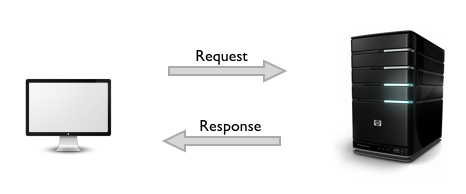
\includegraphics[width=3in]{media/client-server.png}
    \end{center}
\end{frame}

% Slide #6
\begin{frame}{HTTP сообщения}
    Соответственно делятся на 2 типа:
    \begin{itemize}
        \item HTTP запрос
        \item HTTP ответ
    \end{itemize}
    \begin{center}
        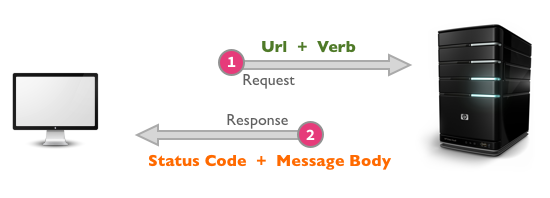
\includegraphics[width=3in]{media/client-server-details.png}
    \end{center}
\end{frame}

% Slide #7
\begin{frame}{Формат сообщения}
    \begin{itemize}
        \item Стартовая строка (обязательное требование)
        \item Заголовки
        \item Пустая строка (только если есть тело сообщения)
        \item Тело сообщения
    \end{itemize}
\end{frame}

% Slide #8
\begin{frame}[fragile]{Пример запроса}
    \begin{Verbatim}[fontsize=\scriptsize]
GET /ru/latest/net/http.html HTTP/1.1
Accept: text/html,application/xhtml+xml,application/xml;q=0.9,*/*;q=0.8
Accept-Language: en-US,en;q=0.5
Connection: keep-alive
Host: lectureswww.readthedocs.org
User-Agent: Mozilla/5.0 (X11; Ubuntu; Linux x86_64; rv:35.0) Gecko/20100101 Firefox/35.0
    \end{Verbatim}
\end{frame}

% Slide #9
\begin{frame}{Стартовая строка запроса}

    GET /ru/latest/net/http.html HTTP/1.1

    Состоит из:
    \begin{itemize}
        \item Метод
        \item URI
        \item HTTP/Версия
    \end{itemize}

    Где:

    \begin{itemize}
        \item Метод — название запроса, одно слово заглавными
            буквами. (GET, POST, PUT, DELETE)
        \item URI определяет путь к запрашиваемому документу.
        \item Версия — пара разделённых точкой цифр. \newline
            Например: 1.0 или 1.1
    \end{itemize}

\end{frame}

% Slide #10
\begin{frame}{Методы}

    Отличаются только! названием! \newline
    Но есть условное разделение:

    \begin{itemize}
        \item GET \--- получить
        \item POST \--- записать
        \item PUT \--- изменить
        \item DELETE \--- удалить
    \end{itemize}

    Пример такого использования RESTfull API

\end{frame}

% Slide #11
\begin{frame}{URL}
    \begin{center}
        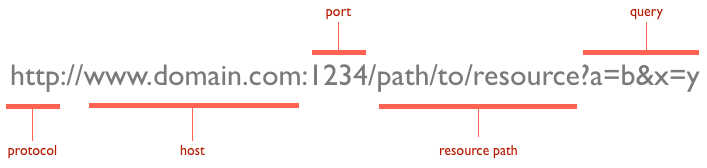
\includegraphics[width=4in]{media/url-structure.png}
    \end{center}
\end{frame}

% Slide #12
\begin{frame}{Заголовки}

    Заголовки выглядят в виде ``key: value''

    \begin{itemize}
        \item Connection: keep-alive
        \item Host: lectureswww.readthedocs.org
        \item User-Agent: Mozilla/5.0
    \end{itemize}

    И делятся на:

    \begin{itemize}
        \item Основные заголовки
        \item Заголовки ответа
        \item Заголовки сущности (запроса)
    \end{itemize}

\end{frame}

% Slide #13
\begin{frame}[fragile]{Пример ответа}
    \begin{Verbatim}[fontsize=\tiny]
HTTP/1.1 200 OK
Server: nginx/1.4.6 (Ubuntu)
Date: Mon, 26 Jan 2015 16:54:33 GMT
Content-Type: text/html
Content-Length: 48059
Last-Modified: Mon, 26 Jan 2015 16:22:21 GMT
Connection: keep-alive
Vary: Accept-Encoding
ETag: "54c669bd-bbbb"
X-Served: Nginx
X-Subdomain-TryFiles: True
X-Deity: hydra-lts
Accept-Ranges: bytes

<!DOCTYPE html>
<!--[if IE 8]><html class="no-js lt-ie9" lang="en" > <![endif]-->
<!--[if gt IE 8]><!--> <html class="no-js" lang="en" > <!--<![endif]-->
<head>
  <meta charset="utf-8">
  <meta name="viewport" content="width=device-width, initial-scale=1.0">
    \end{Verbatim}
\end{frame}

% Slide #14
\begin{frame}{Стартовая строка ответа}

    HTTP/1.1 200 OK

    Состоит из:
    \begin{itemize}
        \item HTTP/Версия
        \item Код состояния
        \item Краткое описание
    \end{itemize}

    Где:

    \begin{itemize}
        \item Версия — как в запросе.
        \item Код состояния (англ. Status Code) — три цифры.
            \newline Например: 200, 301, 404, 500
        \item Пояснение (англ. Reason Phrase) — К коду ответа. Никак не влияет
            на сообщение и является необязательным. (OK, Not Found, Internal Server Error)
    \end{itemize}

\end{frame}

% Slide #15
\begin{frame}[fragile]{Cookie}
    Браузер обычно сохраняет эту информацию на компьютере.\newline
    Например в файл cookies.sqlite. \newline
    И при каждом обращении к сайту передает связанные с ним значения.
    \begin{Verbatim}[fontsize=\small]
HTTP/1.1 200 OK
Content-type: text/html
Set-Cookie: name=value
    \end{Verbatim}
\end{frame}

% Slide #16
\begin{frame}{Cookie}
    Cookie дают возможность организовывать сессии между клиентом и сервером.
\end{frame}

% Slide #17
\begin{frame}{Браузер}
    \begin{center}
        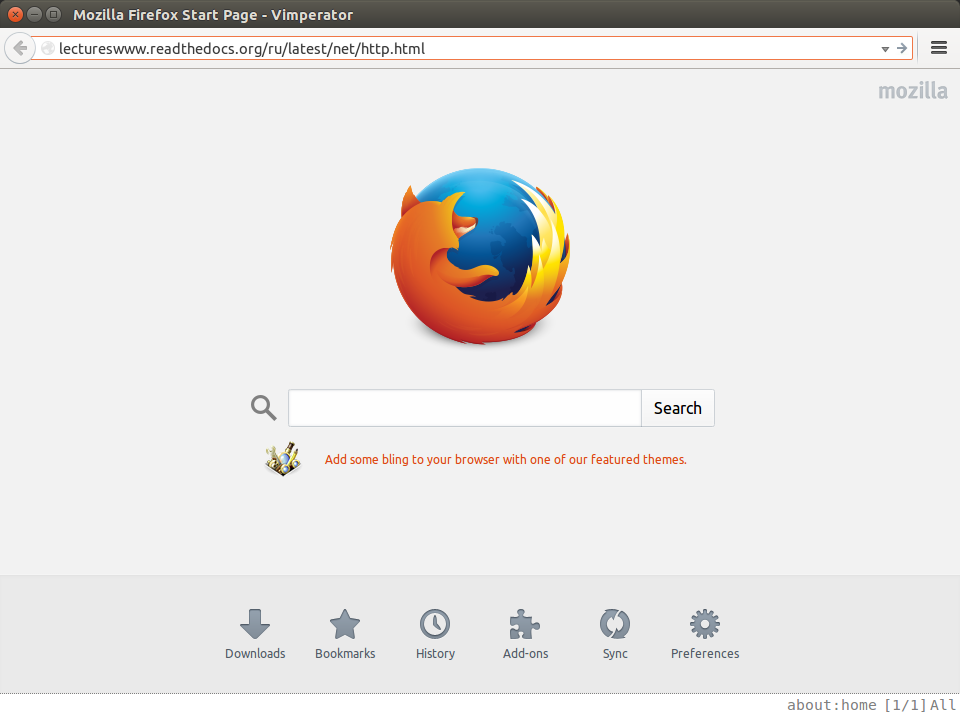
\includegraphics[width=3.5in]{media/http.example.mozzila.png}
    \end{center}
\end{frame}

% Slide #18
\begin{frame}{FireBug}
    \begin{center}
        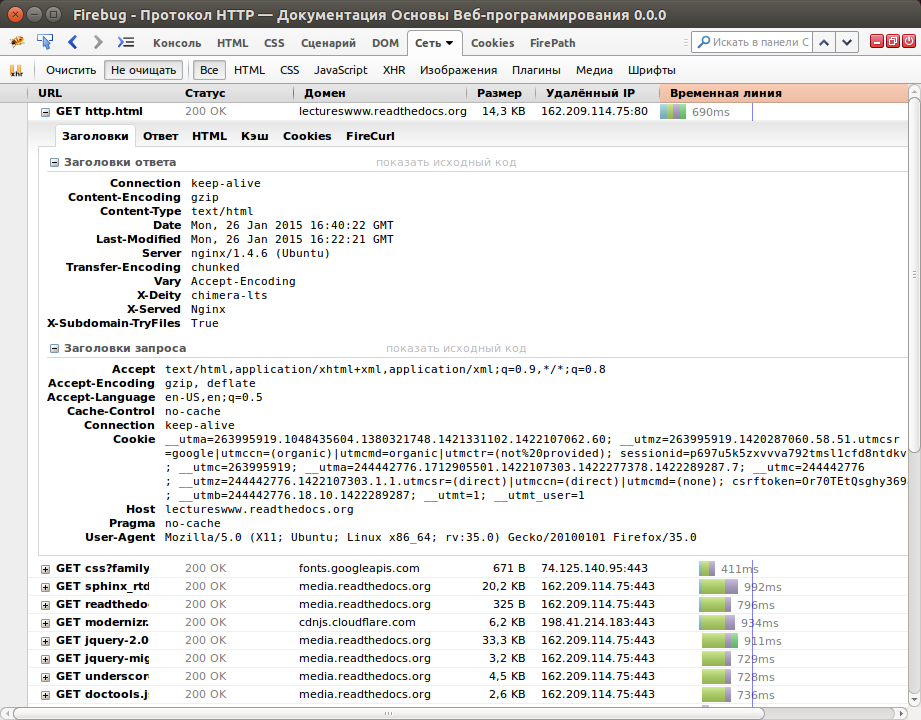
\includegraphics[width=3.5in]{media/firebug1.png}
    \end{center}
\end{frame}

% Slide #19
\begin{frame}[fragile]{telnet}
    \begin{Verbatim}[fontsize=\scriptsize]
$ telnet readthedocs.org 80
Trying 162.209.114.75...
Connected to readthedocs.org.
Escape character is '^]'.
GET /ru/latest/net/http.html HTTP/1.1
Accept: text/html,application/xhtml+xml,application/xml;q=0.9,*/*;q=0.8
Accept-Language: en-US,en;q=0.5
Connection: keep-alive
Host: lectureswww.readthedocs.org
User-Agent: Mozilla/5.0 (X11; Ubuntu; Linux x86_64; rv:35.0) Gecko/20100101 Firefox/35.0
    \end{Verbatim}
\end{frame}

\end{document}
